\documentclass{article}
\usepackage[margin = 1in]{geometry}
\usepackage{graphicx}
\usepackage{booktabs}

\begin{document}

\title{F14-16601: Machine Learning \\ Homework 6 Report}
\author{Dawei Wang \\ {\tt daweiwan@andrew.cmu.edu}}
\maketitle
	
{\bf Code of Conduct Declaration} 	
\begin{itemize}\parskip0pt
	\item I did not receive any help whatsoever from anyone in solving this assignment. 
	\item I did not give any help whatsoever to anyone in solving this assignment. 
\end{itemize}

\vspace{0.5cm}	

Selected $K=169$. See below for the original image and the segmentation result. 
\begin{figure}[h!]
	\centering
	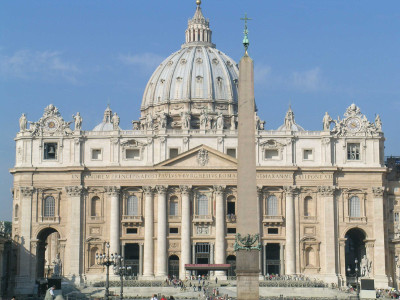
\includegraphics[scale = 0.5]{myBasilica.jpg}\hspace{0.2cm}
	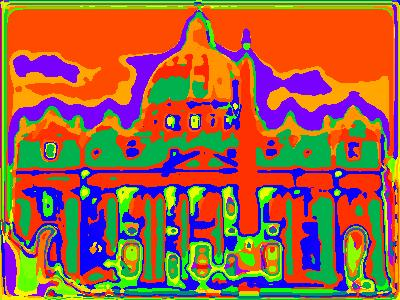
\includegraphics[scale = 0.5]{myBasilicaSegmented.jpg}	
	\caption{St. Peter's Basilica and its Segmentation Result (400x300)} 
\end{figure}

Rationale: 
\begin{itemize}\parskip0pt
	\item I have chosen $K=169$ because $169=13^2$, where $13$ is a prime number. 
	\item I have chosen St. Peter's Basilica because I travelled to there last year. 
\end{itemize}

Performance: 
\begin{table}[h!]
	\centering
	\caption{Elapsed Time}\vspace{4pt}
	\begin{tabular}{lccc} \toprule
		Script & Feature Extraction & K-means & \#Datapoints \\ \midrule
		\tt computeDictionary.m & 173 seconds & $\sim$ 20 seconds & $\sim$21,000 (3\%) \\ 
		\tt segmentation.m & 26.71 seconds & 1.049 seconds & 120,000 \\ \bottomrule
	\end{tabular}
\end{table}

\end{document}